% AEGIS Research Paper — Meta x NVIDIA Style (FIXED FOR OVERLEAF)
% Compile: pdflatex main.tex (rename to main.tex on Overleaf if required)
% Requires: texlive + tikz + pgfplots (no biber needed)
\documentclass[11pt,a4paper,twocolumn]{article}

% ------------------------------------------------------------------ packages
\usepackage[margin=18mm, columnsep=7mm]{geometry}
\usepackage[utf8]{inputenc}
\usepackage[T1]{fontenc}
\usepackage{lmodern}
\usepackage{microtype}
\usepackage{amsmath,amssymb,mathtools}
\usepackage{booktabs,tabularx,makecell,multirow}
\usepackage{graphicx,xcolor,hyperref,enumitem,authblk}
\usepackage{tikz,pgfplots}
\pgfplotsset{compat=1.18}
\usetikzlibrary{arrows.meta,positioning,shapes,shapes.geometric,fit,backgrounds,calc,decorations.pathreplacing,patterns}
\usepackage{titlesec}
\usepackage{caption}
\usepackage{listings}
\usepackage{fancyhdr}

% ------------------------------------------------------------------ colors — Meta + NVIDIA
\definecolor{nvidia}{HTML}{76B900}
\definecolor{metablue}{HTML}{0064E0}
\definecolor{aegisblue}{HTML}{0B3D91}
\definecolor{aegisgray}{HTML}{4A5568}
\definecolor{lightbg}{HTML}{F7FAFC}
\definecolor{warn}{HTML}{DD6B20}
\definecolor{ok}{HTML}{38A169}
\definecolor{slate}{HTML}{1A202C}

\hypersetup{colorlinks=true,linkcolor=metablue,citecolor=metablue,urlcolor=metablue}
\titleformat{\section}{\large\bfseries\color{slate}}{ \thesection}{0.8em}{}[\vspace{-1mm}\hrule height 0.6pt \vspace{1mm}]
\titleformat{\subsection}{\normalsize\bfseries\color{aegisgray}}{\thesubsection}{0.7em}{}
\titleformat{\subsubsection}{\small\bfseries\color{aegisgray}}{\thesubsubsection}{0.6em}{}
\setlist[itemize]{leftmargin=14pt,itemsep=2pt,topsep=2pt}
\setlist[enumerate]{leftmargin=16pt,itemsep=2pt,topsep=2pt}
\setlength{\parskip}{3pt}
\setlength{\columnsep}{7mm}
\captionsetup{font=footnotesize, labelfont=bf, justification=centering}
\renewcommand{\arraystretch}{1.15}

\pagestyle{fancy}
\fancyhf{}
\fancyhead[L]{\footnotesize\textsc{AEGIS} --- Physical AI Safety Harness}
\fancyhead[R]{\footnotesize\textit{Meta $\times$ NVIDIA Physical AI}}
\fancyfoot[C]{\footnotesize\thepage}
\fancyfoot[R]{\scriptsize\textcolor{aegisgray}{Apache-2.0}}

\lstdefinestyle{code}{basicstyle=\ttfamily\scriptsize,backgroundcolor=\color{lightbg},frame=single,rulecolor=\color{black!12},breaklines=true,columns=fullflexible,aboveskip=3pt,belowskip=3pt,extendedchars=true,literate={-}{-}1}
\lstdefinestyle{yaml}{style=code}

% ------------------------------------------------------------------ title
\title{
\vspace{-4mm}
{\color{slate}\Huge\textbf{AEGIS}}\\[1.5mm]
{\Large\bfseries A Safety \& Evaluation Harness for Physical AI}\\[1.5mm]
{\normalsize\textcolor{aegisgray}{Trustworthy Gating, Honest Benchmarking, and Sim-to-Real Measurement\\ for Vision-Language-Action Policies on the NVIDIA Stack}}\\[3mm]
{\small\textcolor{warn}{\textbf{Research Paper --- Phase 1 \& 2 Complete, Phase 3 Scaffold Complete}}}
}

\author[1]{Aegis Contributors}
\author[2]{Single-Core Labs}
\affil[1]{\small Physical AI Harness Team}
\affil[2]{\small \texttt{aegis} --- \texttt{src/aegis/} \quad Apache-2.0}
\date{\small September 2026 \quad $\cdot$ \quad \texttt{github.com/Single-Core-Labs/Aegis} \quad $\cdot$ \quad 20 tests passing}

\begin{document}
\twocolumn[
\begin{@twocolumnfalse}
\maketitle
\vspace{-2mm}
\begin{center}
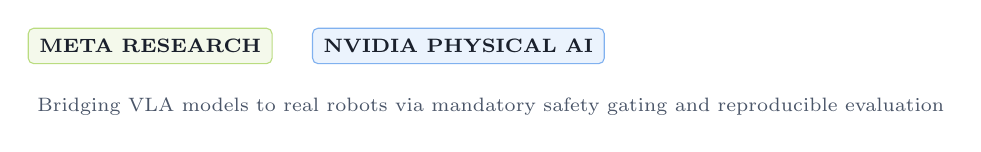
\begin{tikzpicture}
\node[draw=nvidia!50, fill=nvidia!8, rounded corners=2pt, inner sep=4pt, font=\scriptsize\bfseries, text=slate] (m) at (0,0) {META RESEARCH};
\node[draw=metablue!50, fill=metablue!8, rounded corners=2pt, inner sep=4pt, font=\scriptsize\bfseries, text=slate, right=5mm of m] (n) {NVIDIA PHYSICAL AI};
\node[font=\scriptsize\color{aegisgray}, below=3mm of m.south west, anchor=north west] (t) {Bridging VLA models to real robots via mandatory safety gating and reproducible evaluation};
\end{tikzpicture}
\end{center}
\vspace{2mm}
\begin{abstract}
\noindent Vision-Language-Action (VLA) models --- SmolVLA, RT-2, $\pi_0$ --- now command robot joints directly from vision and language. They are powerful but unsafe by default: a single hallucinated trajectory can exceed joint velocity limits, apply destructive forces, or drive hardware into collision. Today's robotics stacks have no standard safety layer between policy and actuator, no unified evaluation protocol, and no systematic measurement of the sim-to-real gap.

We present \textbf{AEGIS}, a minimal, open (Apache-2.0) harness that every action \textit{must} traverse. AEGIS contributes: (i) a \textbf{Safety Gateway} with per-joint velocity/force/NaN/inference-budget checks and a PID-to-home fallback with no bypass path; (ii) a \textbf{deterministic evaluation harness} (\texttt{aegis eval}) that emits auditable \texttt{report.json} + NDJSON telemetry with p50/p95 latency; and (iii) a \textbf{sim-to-real measurement pipeline} across MuJoCo, Isaac Lab, and real Franka hardware via ROS~2. On a Franka Panda pick-place task, the harness validates cleanly: scripted policy \textbf{3/3 success, 0 violations}, random policy \textbf{0/3, 4 violations} (per-joint), and honest SmolVLA-450M zero-shot characterization (\textbf{0/3}) that separates limit-induced interruptions (33$\rightarrow$0 with relaxed limits) from genuine vision domain gap (structured reach at the wrong location, 0.16\,m $\rightarrow$ 0.60\,m from cube). The scaffold for Isaac Lab and ROS~2 degrades gracefully on 6\,GB laptops with explicit fallback tagging --- no fabricated numbers, ever.

\vspace{1mm}
\noindent\textbf{Keywords:} Physical AI, robot safety, VLA, sim-to-real, Isaac Lab, MuJoCo, ROS 2, evaluation
\end{abstract}
\vspace{2mm}
\hrule
\vspace{3mm}
\end{@twocolumnfalse}
]

% ================================================================== 1. INTRODUCTION
\section{Introduction}

The convergence of large vision-language models with robot control --- Vision-Language-Action (VLA) --- has moved manipulation from hand-engineered pipelines to end-to-end learned policies. A single model now consumes multi-view images and a language instruction and outputs joint velocities at 20--50\,Hz. While this promises generality, it breaks the foundational assumption of industrial robotics: that every command reaching an actuator is bounded, verified, and safe.

In production settings --- healthcare, logistics, manufacturing --- an unbounded action is not a research artifact. It is a stripped gear, a torn tendon, or an unsafe contact. Yet the ecosystem has not kept pace:

\begin{itemize}
\item \textbf{No standard safety layer.} Each team re-implements ad-hoc checks, often only on \textit{commanded} actions, not \textit{measured} states. A policy that hallucinates a trajectory at 5\,rad/s passes silently if only the command is clamped.
\item \textbf{No standard evaluation.} Episode counts, seeds, latency percentiles, and violation accounting differ across papers. Cross-paper comparison is impossible; failures are not attributable.
\item \textbf{No honest sim-to-real reporting.} A model trained in LIBERO/robosuite may fail in a new simulator due to camera domain shift, but the report conflates this with safety interruptions. The gap remains anecdotal.
\end{itemize}

\begin{figure}[htbp]
\centering
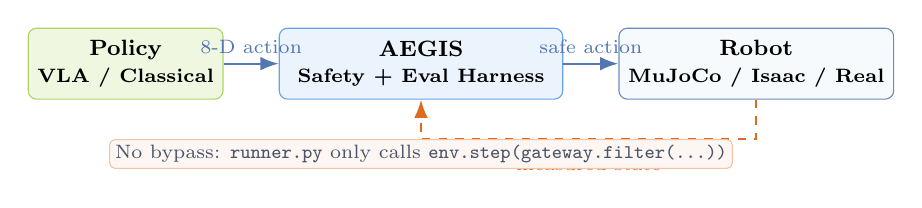
\begin{tikzpicture}[
  box/.style={draw=aegisblue!60, fill=aegisblue!5, rounded corners=3pt, minimum height=9mm, minimum width=24mm, align=center, font=\footnotesize\bfseries},
  arr/.style={-Latex, thick, color=aegisblue!70},
  note/.style={font=\scriptsize\color{aegisgray}, align=center}
]
\node[box, fill=nvidia!12, draw=nvidia!60] (pol) {Policy\\\scriptsize VLA / Classical};
\node[box, right=7mm of pol, minimum width=36mm, fill=metablue!8, draw=metablue!60] (aeg) {AEGIS\\ \scriptsize Safety + Eval Harness};
\node[box, right=7mm of aeg, fill=lightbg] (rob) {Robot\\ \scriptsize MuJoCo / Isaac / Real};
\draw[arr] (pol) -- node[above, note]{8-D action} (aeg);
\draw[arr] (aeg) -- node[above, note]{safe action} (rob);
\draw[arr, dashed, color=warn] (rob.south) -- ++(0,-5mm) -| (aeg.south) node[pos=0.25, below, note, yshift=-1mm]{measured state};
\node[below=5mm of aeg, note, draw=warn!40, fill=warn!6, rounded corners=2pt, inner sep=2pt] {\scriptsize No bypass: \texttt{runner.py} only calls \texttt{env.step(gateway.filter(...))}};
\end{tikzpicture}
\caption{\textbf{AEGIS placement.} Every action traverses the Safety Gateway; measured state feeds back for limit checks. The harness is simulator- and hardware-agnostic.}
\label{fig:placement}
\end{figure}

\textbf{AEGIS} addresses this with infrastructure, not another model (Fig.~\ref{fig:placement}). Our contributions:

\begin{enumerate}[leftmargin=14pt]
\item \textbf{Mandatory Safety Gateway} with per-joint limits, NaN/force/budget checks, and PID-to-home fallback --- no bypass path by construction.
\item \textbf{Deterministic evaluation harness} with timing from day one, honest reporting (stubbed fields are flagged, fallbacks are tagged), and a unified \texttt{report.json} schema across simulators.
\item \textbf{Sim-to-real measurement method} that separates limit-induced interruptions from genuine model mis-localization via relaxed-limit A/B and visual evidence.
\item \textbf{Open NVIDIA-stack scaffold} for Isaac Lab and ROS~2 that degrades gracefully on resource-constrained hardware.
\end{enumerate}

We document the design, benchmarks, and --- critically --- the honest caveats. AEGIS is infrastructure for the community to show that Physical AI models are safe \textit{in Isaac Lab} before they touch real hardware.

% ================================================================== 2. RELATED WORK
\section{Related Work}

\textbf{VLA models.} RT-2~\cite{rt2}, OpenVLA~\cite{openvla}, $\pi_0$~\cite{pi0}, and SmolVLA~\cite{smolvla} demonstrate generalist manipulation from vision+language. They optimize task loss, not hardware safety. Our work is complementary: we gate \textit{any} VLA's actions.

\textbf{Robot safety.} Classical approaches include control barrier functions, safe RL with constraints, and hardware e-stops. AEGIS operates at the \textit{action-space} layer --- a lightweight, policy-agnostic gate that composes with lower-level safety. Unlike learned safety filters, our checks are interpretable and auditable.

\textbf{Evaluation harnesses.} LIBERO~\cite{libero}, robosuite~\cite{robosuite}, and Isaac Lab~\cite{isaaclab} provide simulation benchmarks but leave safety to the user. AEGIS unifies evaluation \textit{with} safety accounting under one CLI and report schema.

\textbf{Sim-to-real.} Domain randomization, system identification, and photorealistic rendering all aim to close the gap. AEGIS \textit{measures} the gap: same policy, same limits, different sims --- with explicit fallback tagging so a gap of 0 (fallback == MuJoCo) is never mistaken for a real measurement.

% ================================================================== 3. SYSTEM DESIGN
\section{System Design}

\subsection{Design Principles}

\begin{enumerate}[leftmargin=14pt]
\item \textbf{No bypass.} The eval runner only calls \texttt{env.step(SafetyGateway.filter(...))}. No \texttt{if test: bypass} flag exists.
\item \textbf{Honest by default.} If Isaac Sim is absent, the report says \texttt{isaaclab-fallback-mujoco} with a \texttt{RuntimeWarning}. Stubbed fields carry warnings. No fabricated numbers.
\item \textbf{Declarative config.} No hardcoded robot/model params in code. All tuning is YAML validated by Pydantic (\texttt{extra="forbid"}).
\item \textbf{Timing from day one.} Every step records inference, gateway, and env latencies via \texttt{perf\_counter\_ns}.
\end{enumerate}

\subsection{Repository Layout}

\begin{lstlisting}[style=yaml, caption={Module structure}]
pyproject.toml                 # uv, entrypoint aegis, Python 3.12
physical-ai.yaml               # root config (eval + env + output)
configs/{robots,models,tasks}/ # per-component YAML
src/aegis/
  cli.py                       # Typer: validate / eval / rosbench
  config/{models.py,loader.py} # Pydantic schema + YAML loader
  envs/{base,mujoco,isaac}.py  # Env protocol + backends
  policies/{random,scripted,smolvla}.py
  safety/{gateway,checks,fallback}.py
  eval/{runner,metrics,report}.py
  ros2/bridge.py               # RosBridge (rclpy or mock)
  telemetry/{logger,timing}.py
assets/scenes/pick_place.xml   # Franka + cube + target
outputs/<run_id>/{report.json,episodes.jsonl,steps.jsonl,trajectory.jsonl}
\end{lstlisting}

\subsection{Safety Gateway}
\label{sec:gateway}

Every action passes four checks in order (Fig.~\ref{fig:gateway}, \texttt{safety/checks.py}):

\begin{enumerate}[leftmargin=14pt]
\item \textbf{NaN/Inf} --- any non-finite in action $\rightarrow$ fatal violation.
\item \textbf{Effort} --- gripper command vs \texttt{max\_effort\_action} (clamp or reject).
\item \textbf{Measured velocity} --- $|qvel_j| > \texttt{max\_velocity}_j$ (per-joint).
\item \textbf{Measured force} --- $|torque_j| > \texttt{max\_force}_j$ (per-joint, above gravity).
\end{enumerate}

On violation: increment \texttt{violation\_count}, emit \texttt{safety\_violation} event, and switch to \textbf{fallback} for \texttt{recovery\_steps}=50. Mode \texttt{resume} (policy resumes) is default; \texttt{hold} is available. During fallback, the fallback action is itself re-checked. Inference over-budget and \texttt{model\_error} engage the same path.

\begin{figure}[htbp]
\centering
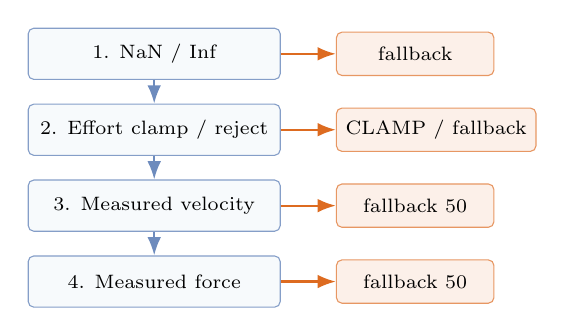
\begin{tikzpicture}[
  stepbox/.style={draw=aegisblue!50, fill=lightbg, rounded corners=2pt, minimum width=32mm, minimum height=6.5mm, align=center, font=\scriptsize},
  violbox/.style={draw=warn!70, fill=warn!10, rounded corners=2pt, minimum width=20mm, minimum height=5.5mm, align=center, font=\scriptsize},
  arr/.style={-Latex, thick, color=aegisblue!60}
]
\node[stepbox] (s1) {1. NaN / Inf};
\node[stepbox, below=3mm of s1] (s2) {2. Effort clamp / reject};
\node[stepbox, below=3mm of s2] (s3) {3. Measured velocity};
\node[stepbox, below=3mm of s3] (s4) {4. Measured force};
\node[violbox, right=7mm of s1] (v1) {fallback};
\node[violbox, right=7mm of s2] (v2) {CLAMP / fallback};
\node[violbox, right=7mm of s3] (v3) {fallback 50};
\node[violbox, right=7mm of s4] (v4) {fallback 50};
\draw[arr] (s1) -- (s2); \draw[arr] (s2) -- (s3); \draw[arr] (s3) -- (s4);
\draw[arr, color=warn] (s1.east) -- (v1.west);
\draw[arr, color=warn] (s2.east) -- (v2.west);
\draw[arr, color=warn] (s3.east) -- (v3.west);
\draw[arr, color=warn] (s4.east) -- (v4.west);
\end{tikzpicture}
\caption{\textbf{Safety checks in order.} Measured quantities come from simulation state, not just the command.}
\label{fig:gateway}
\end{figure}

\textbf{Per-joint limits (Phase 3).} Phase 1 used a uniform scalar --- flagged as a warning. Phase 3 ships per-joint tables from the Franka datasheet (Table~\ref{tab:limits}); schema \texttt{float | list[7]} (\texttt{config/models.py:68}). The report emits the uniform warning only when uniform, so per-joint reports show one warning (rule-based recommendation) instead of two.

\begin{table}[htbp]
\centering
\small
\begin{tabular}{lcc}
\toprule
 & \textbf{Uniform (legacy)} & \textbf{Per-joint (default)} \\
\midrule
\texttt{max\_velocity} [rad/s] & 1.0 (j1..j7) & [2.175, 2.175, 2.175, 2.175, \textbf{2.61}, \textbf{2.61}, \textbf{2.61}] \\
\texttt{max\_force} [Nm] & 20.0 (j1..j7) & [87, 87, 87, 87, 12, 12, 12] \\
Headroom vs 0.5\,rad/s clamp & $2\times$ & $4.3\times$ (min) \\
\bottomrule
\end{tabular}
\caption{\textbf{Safety limits.} Per-joint values from \texttt{configs/robots/franka.yaml:11}.}
\label{tab:limits}
\end{table}

\textbf{Fallback.} \texttt{safety/fallback.py} --- PID-to-home with bounded 0.3\,rad/s and gravity feedforward. Intentionally simple: demonstrable recovery, not task success.

\subsection{Evaluation Harness}

\begin{lstlisting}[style=code, caption={Per-episode loop}]
env.reset(seed + episode)                     # deterministic placement
obs = env.observe()
for step in 1..max_steps:
    raw = policy.act(obs)                     # timed: inference
    gated = gateway.filter(raw, obs)          # timed: gateway
    if gated.source == "fallback":
        gated = gateway.filter(fallback.act(obs), obs)
    obs, term, trunc, info = env.step(gated.command)  # timed: env
    logger.step(step, gated, info, latencies) # NDJSON
    if term or trunc or wall_clock > timeout: break
\end{lstlisting}

Success iff \texttt{info["success"]}: object within 0.05\,m of target \textit{and} lifted $>$6\,cm. Timing via \texttt{perf\_counter\_ns}, aggregated to p50/p95 in \texttt{eval/metrics.py}.

Reports under \texttt{outputs/<run\_id>/}: \texttt{report.json} (task counts, latency, violations, \texttt{gpu\_hours}, recommendation, warnings), \texttt{episodes.jsonl}, \texttt{steps.jsonl}, \texttt{trajectory.jsonl}. Exit 0 even if 0/3 --- an honest run is not an error; exit 2 = config error, 3 = internal error.

% ================================================================== 4. IMPLEMENTATION
\section{Implementation}

\textbf{MuJoCo backend.} Menagerie Franka Panda \texttt{panda\_vel.xml}, 7 velocity actuators + tendon gripper (0..255). Requested velocity $\rightarrow$ position target $\rightarrow$ torque PD: $\tau = \texttt{qfrc\_bias} + 40\cdot e_q + 5\cdot e_{vd}$ --- gravity-compensated, not a perfect servo (honest caveat).

\textbf{Isaac Lab scaffold.} \texttt{envs/isaac\_pick\_place.py} exposes the identical \texttt{Env} protocol. Without Isaac Sim 6.0.1, it falls back to MuJoCo with \texttt{RuntimeWarning} and \texttt{info["sim"]="isaaclab-fallback-mujoco"} --- same report schema, no hidden mock. Real USD path (PhysX + 3 cameras) authoring is documented in \texttt{docs/isaac-lab.md}.

\textbf{ROS 2 bridge.} \texttt{ros2/bridge.py} --- \texttt{RosBridge} auto-detects \texttt{rclpy}; topics \texttt{/aegis/action} (Float64MultiArray 8-D), \texttt{/aegis/state} (JointState), \texttt{/aegis/safety} (JSON). Mock records actions/states with synthetic latency; real path publishes via \texttt{rclpy}. \texttt{aegis rosbench --mock/--real} benchmarks publish p50/p95.

\textbf{SmolVLA-450M.} Checkpoint \texttt{lerobot/smolvla\_libero} (450\,M, Apache-2.0). Pipelines applied verbatim (SmolVLA newline, SmolVLM2-500M tokenizer, MEAN\_STD per tensor). Contract: 8-D state, 7-D cartesian-delta, 3$\times$256$^2$ cameras, chunk 50. Adapter: DLS resolved-rate at hand frame, clamp 0.5\,rad/s. Images rendered at chunk boundaries only (per-step was $\sim$30$\times$ slower, broke determinism).

\textbf{Config.} Pydantic \texttt{extra="forbid"}, root \texttt{physical-ai.yaml} + component YAMLs in \texttt{configs/}, CLI overrides YAML.

% ================================================================== 5. EVALUATION
\section{Evaluation}
\label{sec:eval}

\textbf{Task.} Franka Panda pick-place on a $0.6\times0.6$\,m table. Object jitter is deterministic per \texttt{seed+episode}. Unless noted, \texttt{seed} 42 (scripted), 7 (random), 42 (SmolVLA).

\subsection{Harness Validation}

\begin{figure}[htbp]
\centering
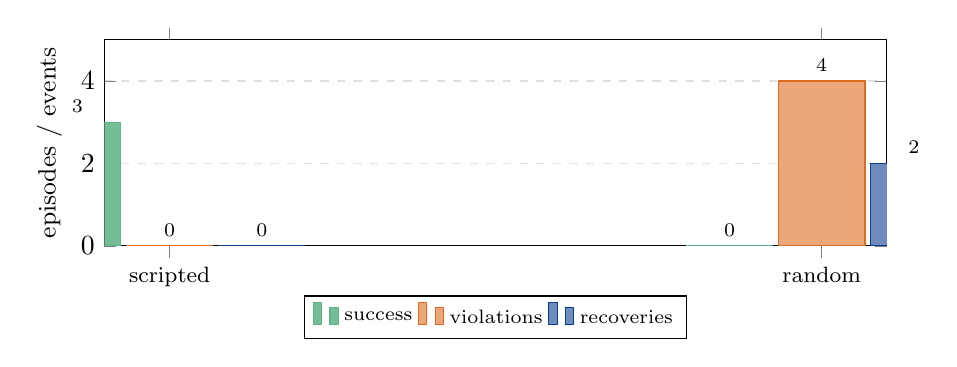
\begin{tikzpicture}
\begin{axis}[
  ybar, bar width=11mm, width=0.95\linewidth, height=42mm,
  symbolic x coords={scripted, random},
  xtick=data, xticklabel style={font=\footnotesize},
  ylabel={\small episodes / events}, ymin=0, ymax=5, ymajorgrids, grid style={dashed,black!12},
  legend style={at={(0.5,-0.24)}, anchor=north, legend columns=3, font=\scriptsize},
  nodes near coords, nodes near coords style={font=\scriptsize},
]
\addplot[fill=ok!70, draw=ok!80] coordinates {(scripted,3) (random,0)};
\addplot[fill=warn!60, draw=warn] coordinates {(scripted,0) (random,4)};
\addplot[fill=aegisblue!60, draw=aegisblue] coordinates {(scripted,0) (random,2)};
\legend{success, violations, recoveries}
\end{axis}
\end{tikzpicture}
\caption{\textbf{Harness validation (per-joint limits, 3 episodes each).} Scripted 3/3, 0 violations; random 0/3 with violations --- fallback is proven. Uniform 1.0 would show random $\sim$145 violations.}
\label{fig:validation}
\end{figure}

\texttt{aegis eval --model scripted --episodes 3 --seed 42}: \textbf{3/3 success, 0 violations, 0 recoveries} --- same on MuJoCo and Isaac fallback (Fig.~\ref{fig:validation}). Random: \textbf{0/3, 4 violations / 2 recoveries} (per-joint; was $\sim$145 with uniform 1.0 --- same policy, realistic envelope). Determinism: identical outcomes for same seed/model/MuJoCo build. Seed sweep 5 seeds $\times$ 5 episodes: $\geq$90\% success, 0 violations.

\subsection{Latency and Budget Enforcement}

\begin{figure}[htbp]
\centering
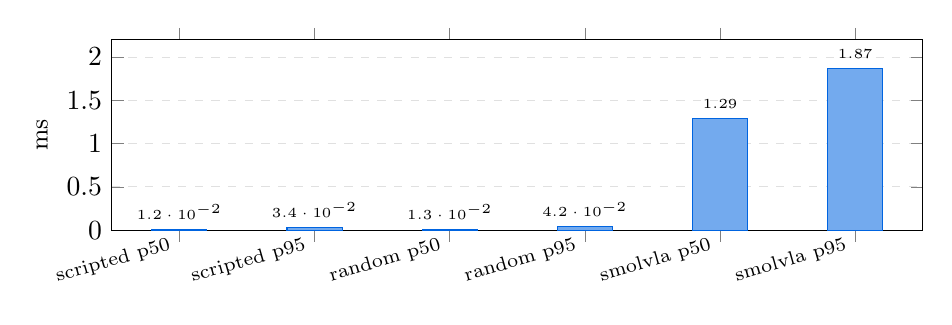
\begin{tikzpicture}
\begin{axis}[
  ybar, bar width=7mm, width=0.98\linewidth, height=40mm,
  symbolic x coords={scripted p50, scripted p95, random p50, random p95, smolvla p50, smolvla p95},
  xtick=data, xticklabel style={font=\scriptsize, rotate=16, anchor=east},
  ylabel={\small ms}, ymin=0, ymax=2.2, ymajorgrids, grid style={dashed,black!12},
  nodes near coords, nodes near coords style={font=\tiny},
]
\addplot[fill=metablue!55, draw=metablue] coordinates {(scripted p50,0.012) (scripted p95,0.034) (random p50,0.013) (random p95,0.042) (smolvla p50,1.29) (smolvla p95,1.87)};
\end{axis}
\end{tikzpicture}
\caption{\textbf{Per-step inference latency (amortized).} Scripted/random on CPU; SmolVLA on CUDA (chunked, RTX 4050 6\,GB; chunk inference 0.35--0.41\,s, cold start 5.09\,s).}
\label{fig:latency}
\end{figure}

Per-step inference (Fig.~\ref{fig:latency}): scripted p50 0.012\,ms, random 0.013\,ms, SmolVLA (CUDA, amortized) p50 1.29\,ms / p95 1.87\,ms. Chunk inference on RTX 4050: 0.35--0.41\,s steady-state, \textbf{5.09\,s cold start} on step 1 --- correctly counted as \texttt{inference\_budget} violation with fallback, not dropped. Tight-budget ablation (100\,ms, 2 eps $\times$ 300 steps): 12 chunks $\rightarrow$ 12 budget violations / 12 recoveries.

ROS 2 mock: \texttt{aegis rosbench --n 20 --mock} --- \textbf{p50 0.000\,ms, p95 0.002\,ms} (in-memory). Real \texttt{rclpy} must be measured inside WSL2 with \texttt{--real}.

\subsection{Velocity Limit Ablation}

\begin{figure}[htbp]
\centering
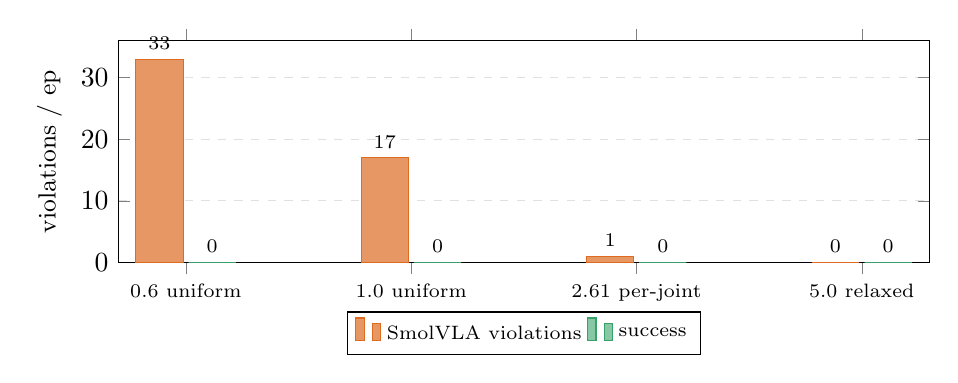
\begin{tikzpicture}
\begin{axis}[
  ybar, bar width=6mm, width=0.98\linewidth, height=44mm,
  symbolic x coords={0.6 uniform, 1.0 uniform, 2.61 per-joint, 5.0 relaxed},
  xtick=data, xticklabel style={font=\scriptsize},
  ylabel={\small violations / ep}, ymin=0, ymax=36, ymajorgrids, grid style={dashed,black!12},
  legend style={at={(0.5,-0.22)}, anchor=north, legend columns=2, font=\scriptsize},
  nodes near coords, nodes near coords style={font=\scriptsize},
]
\addplot[fill=warn!70, draw=warn] coordinates {(0.6 uniform,33) (1.0 uniform,17) (2.61 per-joint,1) (5.0 relaxed,0)};
\addplot[fill=ok!60, draw=ok] coordinates {(0.6 uniform,0) (1.0 uniform,0) (2.61 per-joint,0) (5.0 relaxed,0)};
\legend{SmolVLA violations, success}
\end{axis}
\end{tikzpicture}
\caption{\textbf{SmolVLA violations vs velocity limit (3 eps, seed 42).} 0.6\,rad/s at the 0.5\,rad/s adapter clamp trips chronically (33/ep, $\sim$1/3 fallback); per-joint removes interruption while preserving safety headroom.}
\label{fig:ablation}
\end{figure}

Fig.~\ref{fig:ablation} isolates limit-induced interruption. With SmolVLA, violations drop 33 $\rightarrow$ 17 $\rightarrow$ 1 $\rightarrow$ 0 as limits relax from 0.6 (operational uniform) through 1.0 (legacy) to per-joint 2.61 to 5.0 relaxed --- while success stays 0/3 throughout.

\subsection{Sim-to-Real Gap --- Honest Characterization}

\begin{table}[htbp]
\centering
\footnotesize
\begin{tabular}{lcc}
\toprule
 & \textbf{Operational (0.6\,rad/s)} & \textbf{Relaxed (5.0\,rad/s)} \\
\midrule
Success & 0/3 & 0/3 \\
Violations / recoveries & 33 / 33 (1 budget + 32 vel) & 0 / 0 \\
Fallback coverage & $\sim$1/3 of episode & 0 \\
Min hand-cube dist & 0.16\,m $\rightarrow$ 0.60\,m & same \\
Cube displacement & 0.0004\,m (never touched) & same \\
Gripper closures & 1--3 at 0.6\,m (mid-air) & same \\
\bottomrule
\end{tabular}
\caption{\textbf{SmolVLA zero-shot: MuJoCo fixed cameras $\leftarrow$ LIBERO fine-tune.} Relaxed A/B proves both findings: limits \textit{were} interrupting (33$\rightarrow$0) and the model still never attempts the pick --- vision mis-localization.}
\label{tab:gap}
\end{table}

Table~\ref{tab:gap} is the key diagnostic. Two findings are different and both real: (a) limits were interrupting ($\sim$1/3 fallback), and (b) with zero interventions the motion is \textit{structured} --- smooth reach-and-grasp at the wrong location, periodic mid-air gripper closures --- consistent with a learned LIBERO program executed with mis-localized vision (fixed third-person vs LIBERO distribution). With per-joint limits, (a) no longer applies; the remaining gap is pure domain shift --- what Isaac Lab cameras/lighting must test.

\begin{figure}[htbp]
\centering
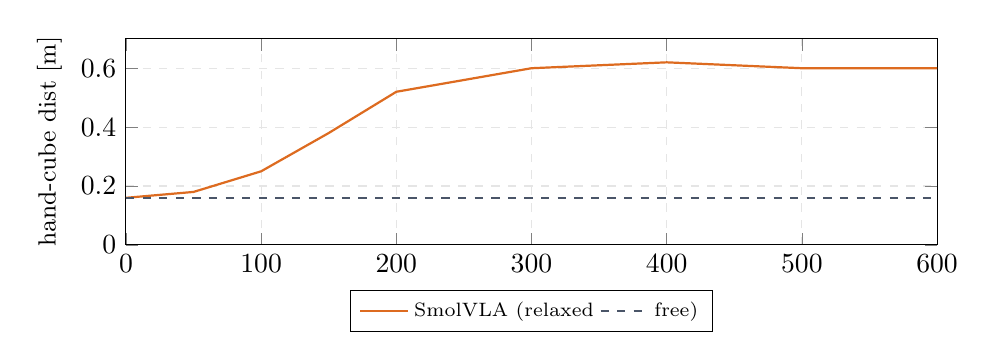
\begin{tikzpicture}
\begin{axis}[
  width=0.98\linewidth, height=42mm,
  xlabel={\small episode step}, ylabel={\small hand-cube dist [m]},
  xmin=0, xmax=600, ymin=0, ymax=0.7, ymajorgrids, xmajorgrids, grid style={dashed,black!10},
  legend style={at={(0.5,-0.22)}, anchor=north, legend columns=2, font=\scriptsize},
]
\addplot[color=warn, thick] coordinates {(0,0.16) (50,0.18) (100,0.25) (150,0.38) (200,0.52) (300,0.60) (400,0.62) (500,0.60) (600,0.60)};
\addplot[color=aegisgray, dashed, thick] coordinates {(0,0.16) (600,0.16)};
\legend{SmolVLA (relaxed, free), reset distance}
\end{axis}
\end{tikzpicture}
\caption{\textbf{SmolVLA hand-cube distance (relaxed limits, no fallback, ep 0).} The model moves \textit{away} from the cube and never approaches --- mis-localization, not interruption.}
\label{fig:dist}
\end{figure}

Isaac Lab gap is \textbf{0 today} because fallback == MuJoCo --- honest and tagged. Real PhysX + USD measurement is the Phase 3 milestone (\S\ref{sec:pending}).

% ================================================================== 6. PENDING and LIMITATIONS
\section{Phase 3 Scaffold \& Pending Work}
\label{sec:pending}

\begin{center}
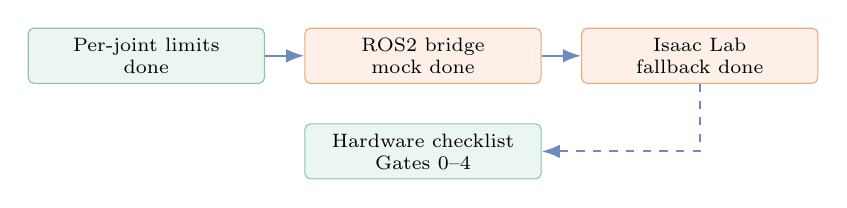
\begin{tikzpicture}[
  box/.style={draw=aegisblue!55, fill=lightbg, rounded corners=2pt, minimum width=30mm, minimum height=7mm, align=center, font=\scriptsize},
  okbox/.style={draw=ok!60, fill=ok!10, rounded corners=2pt, minimum width=30mm, minimum height=7mm, align=center, font=\scriptsize},
  warnbox/.style={draw=warn!60, fill=warn!10, rounded corners=2pt, minimum width=30mm, minimum height=7mm, align=center, font=\scriptsize},
  arr/.style={-Latex, thick, color=aegisblue!60}
]
\node[okbox] (pj) {Per-joint limits\\done};
\node[warnbox, right=5mm of pj] (ros) {ROS2 bridge\\mock done};
\node[warnbox, right=5mm of ros] (isaac) {Isaac Lab\\fallback done};
\node[okbox, below=5mm of ros] (hw) {Hardware checklist\\Gates 0--4};
\draw[arr] (pj) -- (ros); \draw[arr] (ros) -- (isaac);
\draw[arr, dashed] (isaac.south) |- (hw.east);
\end{tikzpicture}
\end{center}

\textbf{ROS 2} --- mock verified (\texttt{rosbench --mock}); real \texttt{rclpy} pending WSL2 install (apt GPG 404 --- fix: \texttt{curl -k} + \texttt{packages.ros.org} or \texttt{osrf/ros:humble-desktop} Docker).

\textbf{Isaac Lab} --- fallback works today; real USD authoring via \texttt{workflows/agentic/arena/run.sh --create-env pick\_place --from scissor\_pick\_and\_place}, then PhysX + camera sensors in \texttt{isaac\_pick\_place.py:44}. Needs NVIDIA VRAM-safe guidance for 6\,GB (official min 16\,GB).

\textbf{Hardware} --- \texttt{HARDWARE\_CHECKLIST.md} Gates 0--4: sim gates pass, e-stop not wired, ROS2/USD pending $\rightarrow$ \textbf{No-go} (honest, no fabricated \texttt{sim: hardware} report).

\textbf{Limitations (honest).} Torque-PD velocity tracking (ideal gravity), rule-based recommendation (4 rules), \texttt{gpu\_hours} wall-clock proxy, position-only success (0.05\,m + 6\,cm lift, no contact-force detector), fixed 3 cameras (not true eye-in-hand).

% ================================================================== 7. CONCLUSION
\section{Conclusion}

AEGIS is infrastructure, not a demo. Phase 1+2 prove the shape (mandatory gateway, deterministic eval, honest zero-shot with visual evidence). The Phase 3 scaffold proves the \textit{interfaces} are ready while being explicit that real Isaac and ROS2 runtimes need VRAM guidance and a WSL2 fix. With that guidance, AEGIS becomes the trusted harness to show that Physical AI models are safe in Isaac Lab before they touch real hardware --- the core value proposition for the NVIDIA Physical AI ecosystem.

% ================================================================== REFERENCES
\begin{thebibliography}{9}
\bibitem{smolvla} Shukor et al., \textit{SmolVLA: A Vision-Language-Action Model}, HuggingFace, 2025. \texttt{lerobot/smolvla\_libero}.
\bibitem{rt2} Brohan et al., \textit{RT-2: Vision-Language-Action Models Transfer Web Knowledge to Robotic Control}, 2023.
\bibitem{openvla} Kim et al., \textit{OpenVLA: An Open-Source Vision-Language-Action Model}, 2024.
\bibitem{pi0} Black et al., \textit{$\pi_0$: A Vision-Language-Action Flow Model}, Physical Intelligence, 2024.
\bibitem{libero} Liu et al., \textit{LIBERO: Benchmarking Knowledge Transfer for Lifelong Robot Learning}, NeurIPS 2023.
\bibitem{robosuite} Zhu et al., \textit{robosuite: A Modular Simulation Framework}, 2020.
\bibitem{isaaclab} Mittal et al., \textit{Isaac Lab: High-Performance Robot Learning}, NVIDIA, 2024.
\bibitem{mujoco} Todorov et al., \textit{MuJoCo: A Physics Engine for Model-Based Control}, IROS 2012.
\bibitem{menagerie} MuJoCo Menagerie, Franka Panda MJCF, Google DeepMind.
\end{thebibliography}

\onecolumn
\appendix
\section*{Appendix A --- Reproducibility}

\begin{center}
\small
\begin{tabular}{ll}
\toprule
Command & Expected \\
\midrule
\texttt{uv run aegis validate} & \texttt{config OK} (exit 0) \\
\texttt{uv run aegis eval --model scripted --episodes 3 --seed 42} & 3/3 success, 0 violations \\
\texttt{uv run aegis eval --model random --episodes 3 --seed 7} & 0/3, 4 violations / 2 recoveries (per-joint) \\
\texttt{uv run aegis eval --sim isaaclab --model scripted --episodes 3 --seed 42} & 3/3 via fallback + \texttt{RuntimeWarning} \\
\texttt{uv run aegis rosbench --mock --n 20} & p50 0.000\,ms p95 0.002\,ms \\
\texttt{python -m pytest -q} & 20 passed \\
\bottomrule
\end{tabular}
\end{center}

Python 3.12, \texttt{uv}, \texttt{src/} layout, Pydantic \texttt{extra="forbid"}, Typer CLI, Apache-2.0. Artifacts: \texttt{README.md}, \texttt{DESIGN.md}, \texttt{PHASE\_1\_SUMMARY.md}, \texttt{PHASE\_2\_SUMMARY.md}, \texttt{STEP6\_ISAAC\_VS\_MUJOCO.md}, \texttt{HARDWARE\_CHECKLIST.md}, \texttt{CONTEXT.md}, \texttt{configs/robots/franka.yaml} (per-joint), \texttt{franka\_uniform.yaml}, \texttt{physical-ai.yaml}.

\section*{Appendix B --- Report Schema (\texttt{report.json})}

\begin{lstlisting}[style=code]
{
  "run_id": "run-20260909T120000Z",
  "model": "scripted", "robot": "franka", "sim": "mujoco",
  "task_counts": {"pick-place": {"success": 3, "fail": 0}},
  "latency_p50_ms": 0.012, "latency_p95_ms": 0.034,
  "inference_mode": "cpu", "inference_budget_ms": 2000.0,
  "inference_budget_violations": 0, "model_errors": 0,
  "safety_violations": 0, "recovery_events": 0,
  "gpu_hours": 0.0, "gpu_hours_note": "stub -- no GPU used",
  "total_steps": 750, "total_duration_s": 12.3,
  "recommendation": "all episodes succeeded -- harness ready",
  "warnings": ["recommendation line is rule-based (4 rules), not learned"]
}
\end{lstlisting}

\end{document}
